%
% http://www.ulb.ac.be/di/info-f101/Projets/08-09/projet4.pdf
%

\documentclass[a4paper, 10pt]{article}
\usepackage{a4wide}
\usepackage {amsmath}
\usepackage {graphicx}
\usepackage[utf8]{inputenc} 
\usepackage[francais]{babel}
\usepackage{fancyhdr}
\usepackage{setspace}
\usepackage{fancyhdr}
\usepackage{lastpage}
\usepackage{extramarks}
\usepackage{chngpage}
\usepackage{soul}
\usepackage[usenames,dvipsnames]{color}
\usepackage{graphicx,float,wrapfig}
\usepackage{ifthen}
\usepackage{listings}
\usepackage{courier}
\usepackage{color}
\usepackage{xcolor}
\usepackage{esint}
\usepackage{pdfsync}

\usepackage{listings, color, setspace, graphics}
\usepackage{fancyhdr, amsmath, amssymb, setspace, amssymb}
\usepackage{pdfpages}
\usepackage{filecontents}

\definecolor{dkgreen}{rgb}{0,0.6,0}
\definecolor{gray}{rgb}{0.5,0.5,0.5}
\definecolor{mauve}{rgb}{0.58,0,0.82}

\lstset{language=C++,
numbers=left, 
 stepnumber=1,
 showstringspaces=false,   
showspaces=false, 
frame=single,
keywordstyle=\color{blue}
}       

\newcommand{\mylisting}[2][]{%
    \lstinputlisting[caption={\texttt{\detokenize{#2}}},#1]{#2}%
}


\lhead{} 
\chead{} 
\rhead{\bfseries Python} 
\lfoot{L Bastard \& JC Toussaint}
%\cfoot{} 
%\rfoot{\thepage}

\begin{filecontents*}{test.cc}

\end{filecontents*}


\pagestyle{fancy}

\begin{document}

\title{01 - Le projet PGM}

\author{Lionel Bastard \& Jean-Christophe Toussaint\\
%  Phelma\\
% \texttt{prenom.nom@phelma.grenoble-inp.fr}
}
\date{\today}
 
\maketitle


Le but de ce projet est de développer une application qui permet de lire, écrire et manipuler des images au format PGM.


\section{Introduction}

Une image peut être stockée sous la forme d'un tableau de points élémentaires appelés pixels (abréviation de picture elements). On s'intéressera dans un premier temps à la manipulation d'images
 en niveaux de gris (ou grayscale en anglais), c’est-à-dire, des images dont les ''couleurs'' sont uniquement des nuances de gris. On peut représenter une telle image par une matrice d’entiers, dont la valeur des éléments représente l’intensité lumineuse des pixels de l’image. Par conséquent, un traitement d’image peut être réalisé en manipulant 
 la matrice qui la représente.
 
\section{Fichier PGM}

Un fichier PGM (Portable Gray Map) est composé de deux parties : 
\begin{enumerate}
\item Un entête indiquant les paramètres de l'image
\item Une matrice dont chaque élément représente le niveau de gris d’un pixel de l’image.
\end{enumerate}
 L’entête contient 3 lignes. La première ligne est toujours la même, il s’agit de l’identifiant du fichier PGM : P2 pour une image codée en ASCII et P5 pour une image codée en binaire. La seconde ligne contient 2 entiers séparés par un espace: le nombre de colonnes et le nombre de lignes de pixels de l’image. 
 \begin{figure}[h!]
\begin{center}$
\begin{array}{c}
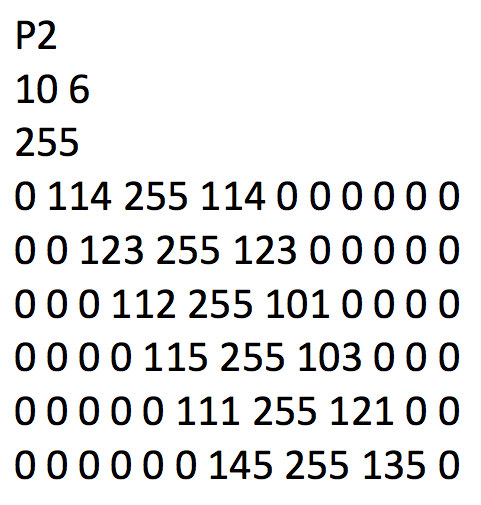
\includegraphics[scale=1, width=5cm]{example_pgm.png} 

\includegraphics[scale=1, width=6cm]{example_screen.png} 
\end{array}$
\end{center}
\label{ExamplePGM} 
\caption{Exemple de fichier PGM et image associée.  }
\end{figure}

 Enfin, la troisième ligne contient la valeur maximale que peut prendre un pixel (par exemple : 255 pour un codage des niveaux de gris entre 0 et 255). 
 Les lignes qui suivent donnent l’intensité de chaque pixel. Ceux-ci sont énumérés ligne par ligne et colonne par colonne. Ainsi la première valeur est l’intensité du pixel du coin supérieur gauche, la seconde est l’intensité du pixel de la première ligne, deuxième colonne, etc.

Par exemple, un fichier PGM contenant les informations ci-dessous est l’encodage d’une image représentant une barre oblique blanche sur fond noir (voir Fig. 1). 



\section{Organisation du programme}

Pour travailler sur une image (modifier la valeur des pixels pour changer le contraste de l'image par exemple), il est nécessaire de dissocier deux entités :
\begin{enumerate} 
\item Le fichier contenant l'image, qui est stocké sur disque dur.
\item La représentation en mémoire de l'image, qui est stockée dans la mémoire vive allouée au programme. C'est sur cette représentation mémoire que l'on effectuera toutes les manipulations de l'image. Une fois l'image modifée à notre convenance, il sera possible de la stocker dans un fichier via une fonction dédiée.
\end{enumerate} 

Dans ce projet, vous stockerez l'image en mémoire sous la forme d'un tableau numpy 
de taille NROWS $\times$ NCOLS où NROWS est le nombre de pixels en largeur et NCOLS celui
en hauteur. Ce tableau comprendra l'ensemble des pixels de l'image. 
Par ailleurs, pour minimiser la place mémoire, le tableau sera constitué d'élément du type {\tt uint8}, qui occupent un octet de mémoire seulement. 
Seules des images contenant au maximum 256 niveaux de gris pourront donc être traitées par notre programme. Le code suivant donne un exemple de création et d'utilisation du tableau contenant les valeurs des pixels de l'image.

On rappelle que
\begin{enumerate}  
\item  A=np.zeros(shape=(NROWS, NCOLS), dtype='uint8')
crée un tableau de zéros,
\item  U=A.astype(np.uint8) force la conversion de type
d'un tableau de réels $R$ en un d'entiers non signés U.
\end{enumerate} 

Votre programme devra lire et écrire des images au format PGM au format ASCII (texte).
Dans le fichier ASCII de l'image, les données de l'intensité lumineuse des pixels sont 
écrites sous forme d'un entier, 
chaque entier étant séparé par un espace  vide au moins, et chaque ligne de l'image étant séparée par un retour à la ligne.

\section{Travail à réaliser}
On vous demande d'écrire sous Spyder, l'ensemble de fonctions suivantes permettant de générer, lire, écrire et manipuler les images au format PGM.

\subsection{Version scalaire}
\begin{enumerate} 
\item créer une fonction {\tt fun(x, y)} qui à partir d'un couple de réels (x, y) 
retourne l'évaluation de $\frac{1}{2} (\sin(x)\; \sin(y)+1)$.
La valeur retournée est dans $[0, 1]$.

\item créer une fonction {\tt centering(i, L)} qui à partir de deux entiers $i$ et $L$
retourne $2 i/L-1$. La fonction vérifiera que $i \in [0, L[$. \\
On pourra mettre en oeuvre l'instruction suivante : \\
{\tt assert condition, "out of range"} en adaptant la condition à votre usage.

\item créer une fonction {\tt createImg(fun, NROWS, NCOLS, NLEVELS=255)}
qui retourne un tableau numpy {\tt img} de taille NROWS $\times$ NCOLS contenant les valeurs
des pixels comprises entre 0 et 255. \\
Pour tout couple d'indice $(i, j) \in [0, NROWS[ \times [0, NCOLS[$, définir
{\tt x=$\pi$ centering(i, NROWS)} et {\tt y=$\pi$  centering(j, NCOLS)}
et stocker dans l'élément $(i, j)$ la valeur de {\tt NLEVELS $\times$ fun(x, y)}
dont on ne gardera que la partie entière. Pour ce faire utiliser la fonction $\tt floor$
du module math.

\item créer une fonction {\tt writeImg(img, filename)} qui sauvegarde
dans le fichier {\tt filename} l'image {\tt img} au format $PGM$ ASCII.

\item Proposer un petit programme test sur une petite image. Vérifier
avec un éditeur de texte que le fichier a la bonne structure.
Tester-le en prenant des valeurs de NROWS et NCOLS différentes!

On pourra utiliser un petit programme comme OpenSeeIt sous windows ou eog
sous linux pour visualiser l'image stockée.

%\item création d'une fonction {\tt readImg(filename)} qui lit  le fichier PGM {\tt filename}
%et qui retourne un tableau numpy {\tt img} contenant l'intensité de chaque pixel.

\item Un de vos collègues vous a fourni une fonction {\tt readImg(filename)}
qui lit  le fichier PGM {\tt filename}
et qui retourne un tuple, en omettant de la documenter ! A vous de le faire
maintenant.

\begin{lstlisting}[language=python]
def readImg(filename):
    with open(filename) as f:
        lines = f.readlines()

#to be commented
    for l in list(lines):
        if l[0] == '#':
            lines.remove(l)    

#to be commented
    assert lines[0].strip() == 'P2' 

#to be commented
    data = []
    for line in lines[1:]:
        data.extend([int(c) for c in line.split()])

#to be commented
    return (np.array(data[3:]),(data[1],data[0]),data[2])
\end{lstlisting}

Quelle est la structure du tuple retourné? Où se trouve le tableau
contenant l'image, quelles sont ses dimensions?
A quoi correspond le triplet (data[1],data[0]),data[2]) ?

\item Compléter le programme test en lisant une image PGM stocker dans un fichier
en utilisant  la fonction précédente {\tt tup = readImg(filename} puis
en insérant la portion de code suivante :
\begin{lstlisting}[language=python]
plt.imshow(np.reshape(tup[0],tup[1]), cmap=cm.jet) 
plt.colorbar()
plt.show()
\end{lstlisting}
N'oublier pas d'insérer en tête de programmes les modules suivants:
\begin{lstlisting}[language=python]
import matplotlib.pyplot as plt
import matplotlib.cm as cm   # colormap
\end{lstlisting}

En vous référant à la documentation de la fonction {\tt plt.imshow},
expliquer que fait la fonction numpy {\tt np.reshape(tup[0],tup[1])}?

\item On désire mesurer le temps CPU nécessaire pour générer une image
de taille 512 $\times$ 512. Utiliser la portion de code suivant :
\begin{lstlisting}[language=python]
from time import process_time

# Start the stopwatch / counter 
t1_start = process_time() 
   
Z=createImg(fun, NROWS, NCOLS)
  
# Stop the stopwatch / counter
t1_stop = process_time()
print("Elapsed time (s):", t1_stop-t1_start) 
\end{lstlisting}

\end{enumerate} 

Noter le temps écoulé.
\subsection{Version vectorielle}

On complète notre programme test avec des versions vectorisées des
fonctions {\tt fun} et {\tt createImg}.

\begin{enumerate} 

\item créer une fonction {\tt createImgVec(funvec, NROWS, NCOLS, NLEVELS=255)}
qui utilisera la fonction numpy {\tt np.meshgrid(x, y)} où
x est un tableau numpy de NROWS valeurs équi-espacées entre $[-\pi,\pi]$
et y de NCOLS valeurs équi-espacées entre $[-\pi,\pi]$.
La fonction {\tt funvec} mettra en oeuvre les versions vectorielles numpy de
la fonction sinus. 

La documentation de {\tt np.floor} nous informe que la valeur retournée est un réel.
L'image étant codée avec des entiers non signés 8 bits,
il faut donc convertir le type en utilisant la méthode {\tt astype}, vue dans la
section 3.

\item mesurer de nouveau le temps écoulé pour créer une image de taille 512 $\times$ 512
avec la fonction {\tt createImgVec}. Que remarquez-vous?

\item développer une fonction de seuillage {\tt threshold(img, seuil)} où seuil
est un entier compris entre 0 et NLEVELS. Cette fonction remplace toute valeur
supérieure au seuil par cette valeur de seuil. 
Montrer qu'il est possible d'écrire le corps de cette fonction en une ligne.
{\it indication : faire une recherche sur internet en tapant numpy array with condition.}

\end{enumerate}

\subsection{BONUS : stockage des images en format binaire 'P5'}

On dupliquera le projet précédent avant de modifier toutes fonctions.

\begin{enumerate} 

\item On désire modifier la fonction   {\tt writeImg(img, filename)}  pour stocker l'image en niveau de gris 
dans un fichier au format binaire 'P5'. 

Pour écrire l'entête ASCII du fichier, on utilisera la fonction python
{\tt open(filename, 'w')} en mode écriture ({\bf w}rite). Puis,  on le reouvrira en mode ajout ({\bf a}ppend) avec la fonction python
{\tt open(filename, 'ab')} pour le compléter. Noter que la conversion d'une variable numérique z en octets peut être
réalisée avec la fonction membre {\tt z.to\_bytes}.

\item Proposer un petit programme test sur une petite image. 

\item On désire modifier la fonction {\tt readImg(filename)} qui lit  le fichier PGM {\tt filename}
au format binaire 'P5'. Noter que la conversion d'octets en valeur numérique peut être effectuée avec la fonction
membre  {\tt int.from\_bytes}.

\end{enumerate}

\end{document}

